% SPDX-FileCopyrightText: 2024 Lukas Zirpel <thesis+lukas@zirpel.de>
% SPDX-License-Identifier: GPL-3.0-only

\chapter{Results}
\label{chap:results}

This chapter presents the results obtained from our experiments.
We analyze the impact of the censorship evasion protocols on key network metrics relevant to their practical deployment and effectiveness.
Specifically, we examine the protocols' influence on packet size and transmission efficiency, considering factors such as overhead and maximum transmission unit.
We also investigate the resource utilization of each protocol, including processing power and memory consumption.
The results are organized to provide a comprehensive analysis of the protocols' performance characteristics, ultimately providing insights into their suitability for real-world censorship circumvention scenarios.


\section{Evaluation of Selected Protocols: Implementation and Challenges}
Running iperf3 with no protocol and with WireGuard worked out of the box.
The same was not true for the other protocols.

We were unable to evaluate \textbf{ICMPTX}.
The program has a bug, where it crashes almost immediately after iperf3 starts sending data through the tunnel.
It fails with the error message \texttt{sendto: No buffer space available}.
The issue was mentioned previously \cite{icmptx-sendto-no-buffer-space-avaiable}.
The maintainer proposed two workarounds but using either one alone or both at the same time did not resolve the issue.
The code of our attempts at workarounds can be found in commit \texttt{d96d541f8b81ae5a9c68804785d35f9cb8eafe0b}.
The problem seems to occur when trying to send data into the tunnel at a faster rate than the underlying link can support.
Tunnel software should be able to handle this case by dropping packets instead of crashing.
All other tunnel protocols we tested handled this case gracefully.
We did not find this problem while experimenting with VMs since the VMs are connected using a virtual 1Gbit/s network, while iperf3 is configured to only send data at a rate of 100Mbit/s.
Even with overhead caused by ICMP and other headers, the data rate does not come close to the 1Gbit/s supported by the virtual network, so the situation described above does not occur.

The theoretical throughput of \textbf{iodine} is limited by its design, which allows only one packet to be in flight at a time \cite{iodine-README}.
This suggests that the achievable throughput is directly dependent on the network latency and should be generally low.
The authors claim a maximum downstream bandwidth of 1 Mbit/s \cite{iodine-homepage}.
However, our observed data rates are much higher than initially expected (see \Cref{fig:graph-5-iodine-constant-throughput}), indicating that this limitation may no longer apply.
We confirm this theory by looking at the stream of packets with Wireshark.
It may also apply only to one direction of the communication but we did not test this.
Reliable measurement of directional throughput would require an improved setup, see \Cref{fig:optimal_network_schematic}.
iodine was very flaky in our testing, with its connection frequently breaking and the throughput dropping to zero.
After a minute the client exits with \texttt{iodine: No downstream data received in 60 seconds, shutting down.}.
There are no other error messages on the client or server.
This can even happen when we do not introduce any artificial loss, delay or duplicate packets (tested with an IP payload size of 1260 bytes).
systemd subsequently restarts the process and a new connection is established.
We acknowledge that trying to send 100Mbit/s of data through a DNS tunnel is unrealistic when iodine only keeps one packet in flight at a time and claims a maximum downstream bandwidth of 1 Mbit/s.
But this should only result in severe packet loss and not cause the tunnel connection to break.
In \Cref{fig:graph-2-iodine-dropout-packets} all data transfer stops shortly after the start of the test and then resumes after about eight seconds.
\begin{figure}[tbh]
	\centering
	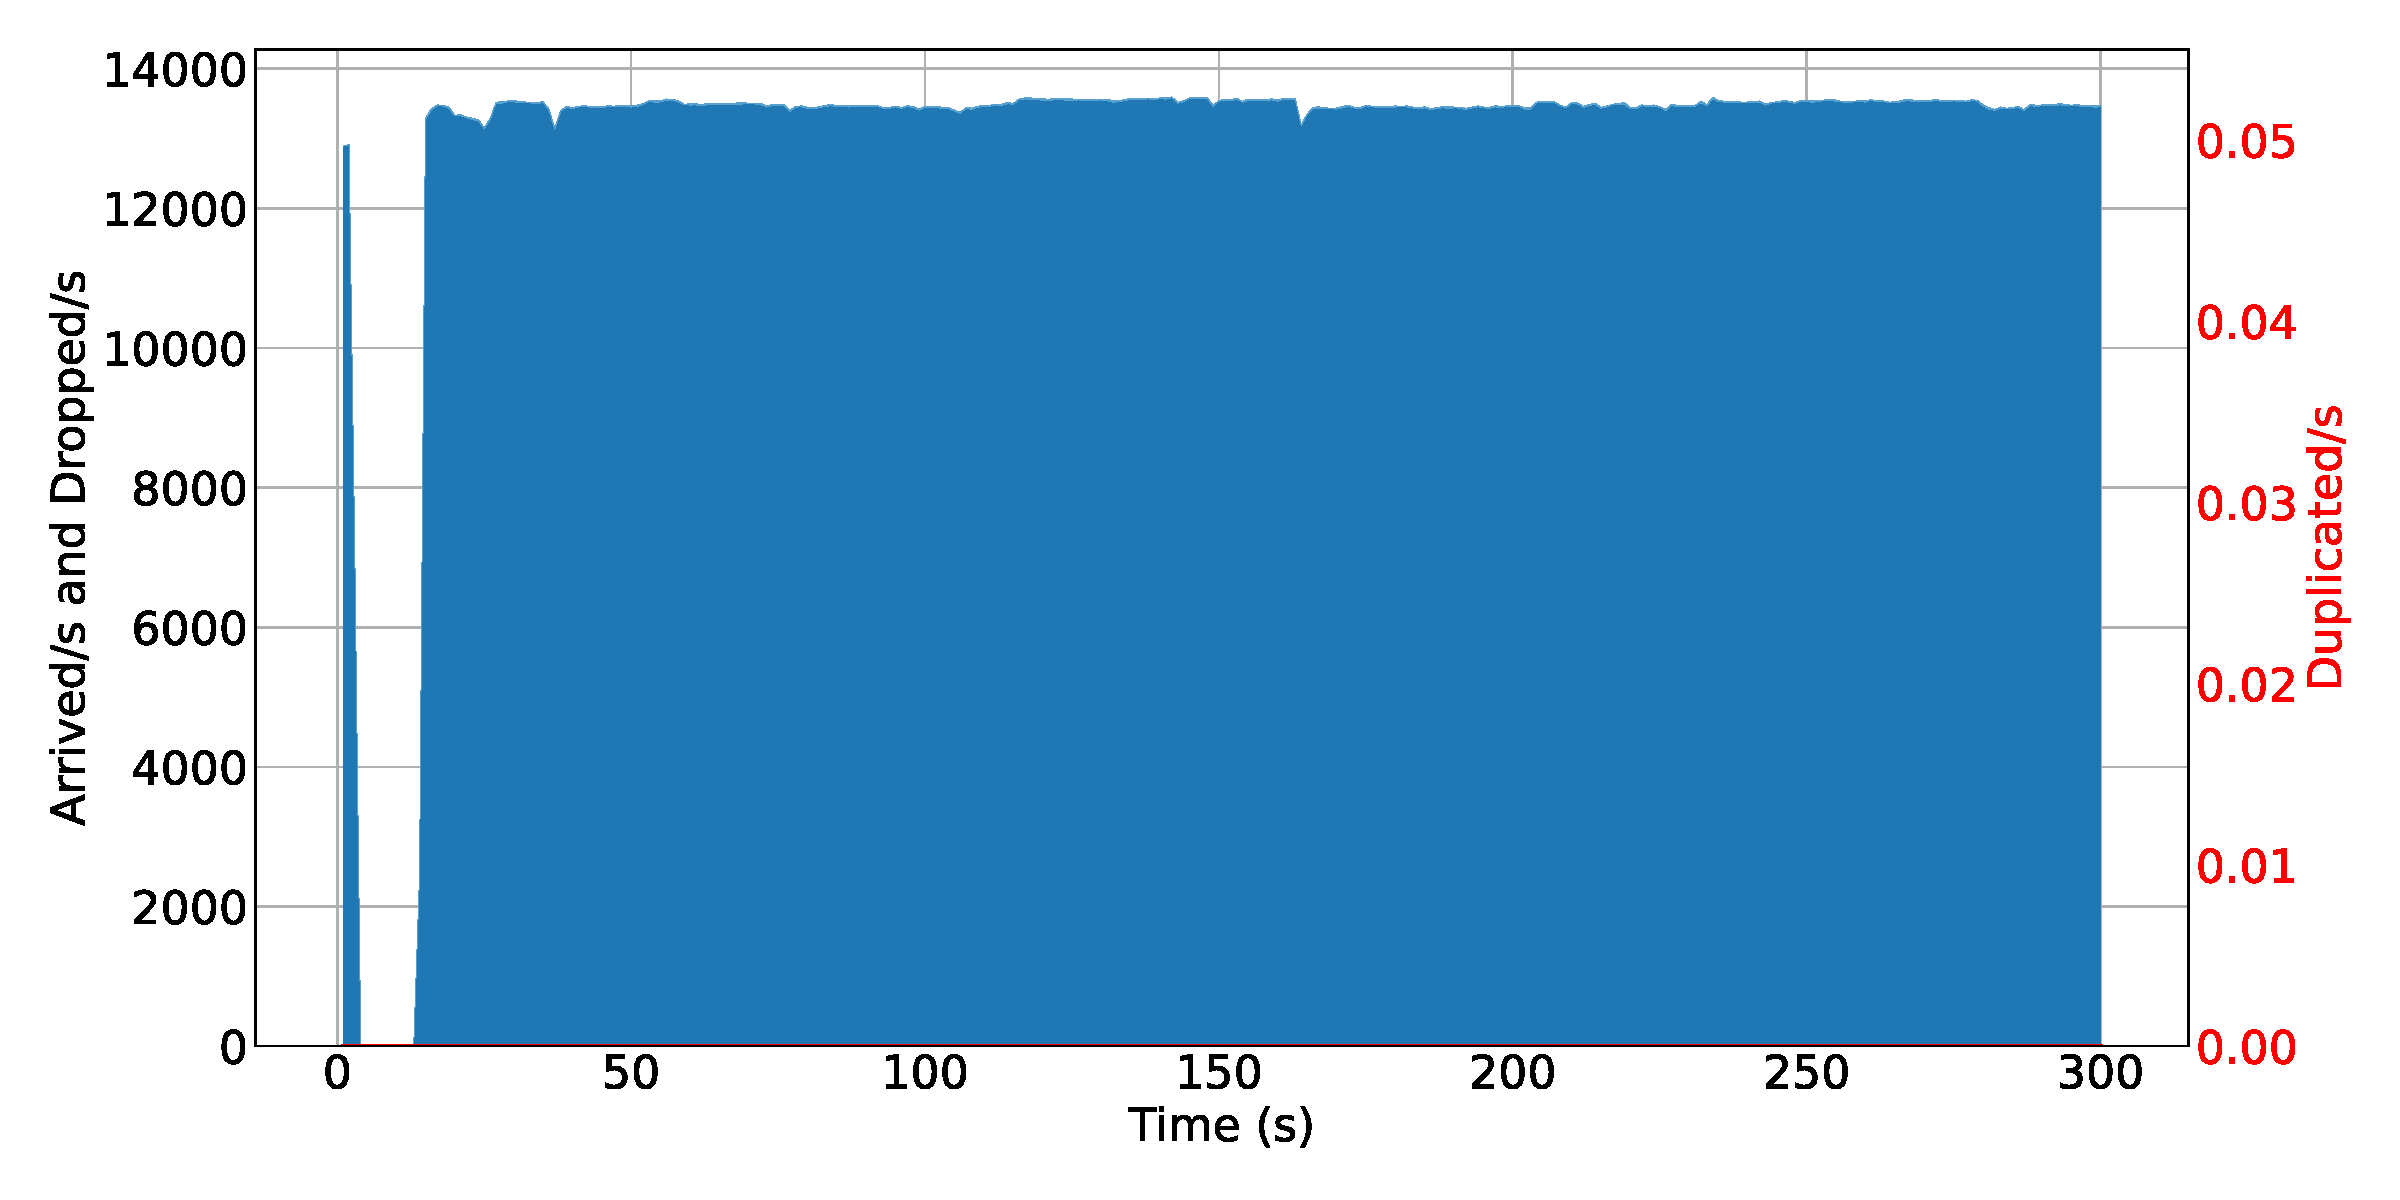
\includegraphics[draft=false,width=0.9\textwidth]{figures/Graphs/graph-2-iodine-dropout/packet_counts_all.pdf}
	\caption{Number of packets per second, iodine, 1260 IPv4 payload size, 0.1\% loss}
	\label{fig:graph-2-iodine-dropout-packets}
\end{figure}

\begin{figure}[tbh]
	\centering
	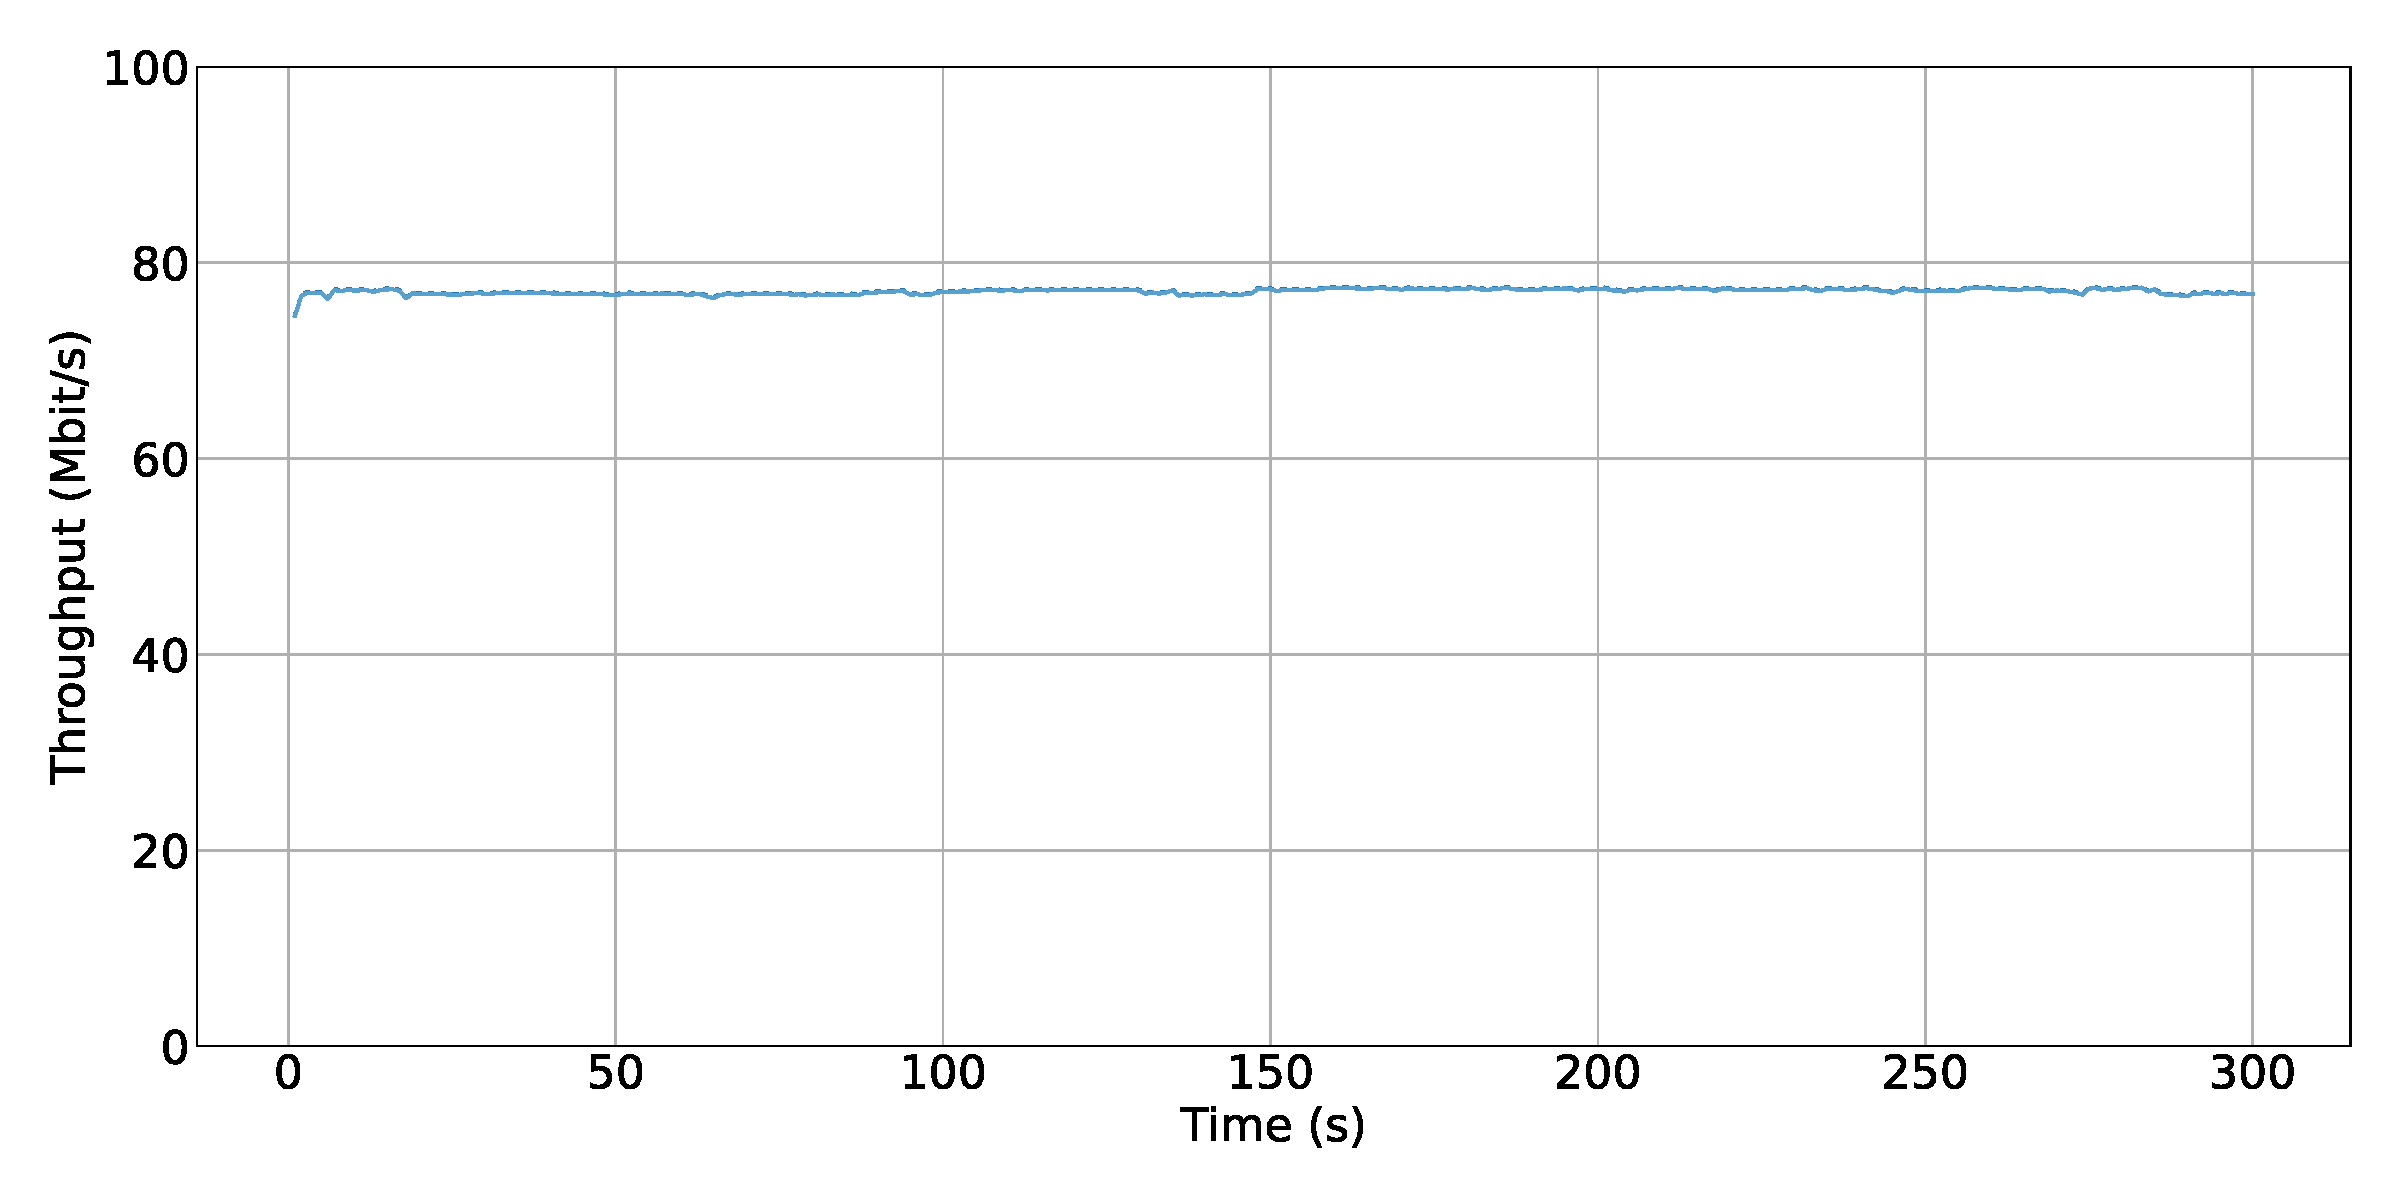
\includegraphics[draft=false,width=0.9\textwidth]{figures/Graphs/graph-5-iodine-constant-throughput/throughput.pdf}
	\caption{Throughput with overhead, iodine, 1400 IPv4 payload size, 0.1\% loss}
	\label{fig:graph-5-iodine-constant-throughput}
\end{figure}


\textbf{Tor Pluggable Transports}, such as obfs4 and Snowflake, are primarily designed for stream-oriented data, typically using TCP.
Because our tests use UDP packets, we are unable to evaluate the performance of these protocols under their intended operating conditions.
A different test setup employing a connection-oriented data stream (TCP) would be necessary for a more accurate assessment.
However, the congestion control algorithm may then influence the results.
Alternatively, using a UDP-over-TCP tunnel might also work.


\noindent\textbf{General Observations:}
For the majority of protocols tested, the observed latency, packet loss, and duplication closely matched the values configured in the network emulator (tc-netem).
The measured throughput is predictably influenced by the number and size of transmitted and dropped packets.

We measure a small percentage (~0.001\%) of packets which seem to have a negative latency.
The biggest time difference is in the single digit millisecond range.
We are not sure what causes this but it indicates that our packet time stamps are slightly noisy with the most extreme outliers being off by several milliseconds.


\subsection{Data Visualization}
\subsubsection{Single Measurement Graphs (Detailed View):}
\label{sect:graphs-single}
These graphs provide a detailed view of a single measurement, allowing us to assess its consistency over time.
Each graph is plotted against time, divided into one second buckets.
An example can be found in \Cref{fig:graph-5-iodine-constant-throughput}.

\noindent\textbf{Latency:} A box plot is used to show the distribution of latency within each time bucket.
This visualization helps identify not only the average latency but also the range and variability (including outliers or "tail latency") within each bucket.

\noindent\textbf{Packet Counts:} A stackplot shows how many packets were sent and how many of them arrived at the other side of the router.
A line graph shows the number of duplicated packets.
This allows us to track packet counts over time and identify any fluctuations or drops.

\noindent\textbf{Throughput:} A line graph shows the throughput achieved in each time bucket.
This graph helps visualize the consistency of throughput over the duration of the measurement.


\subsubsection{Multi-Measurement Graphs (Parameter Influence):}
\label{sect:graphs-multi}
These graphs compare multiple measurements to visualize the influence of a specific parameter.

\begin{figure}[t!]
	\centering
	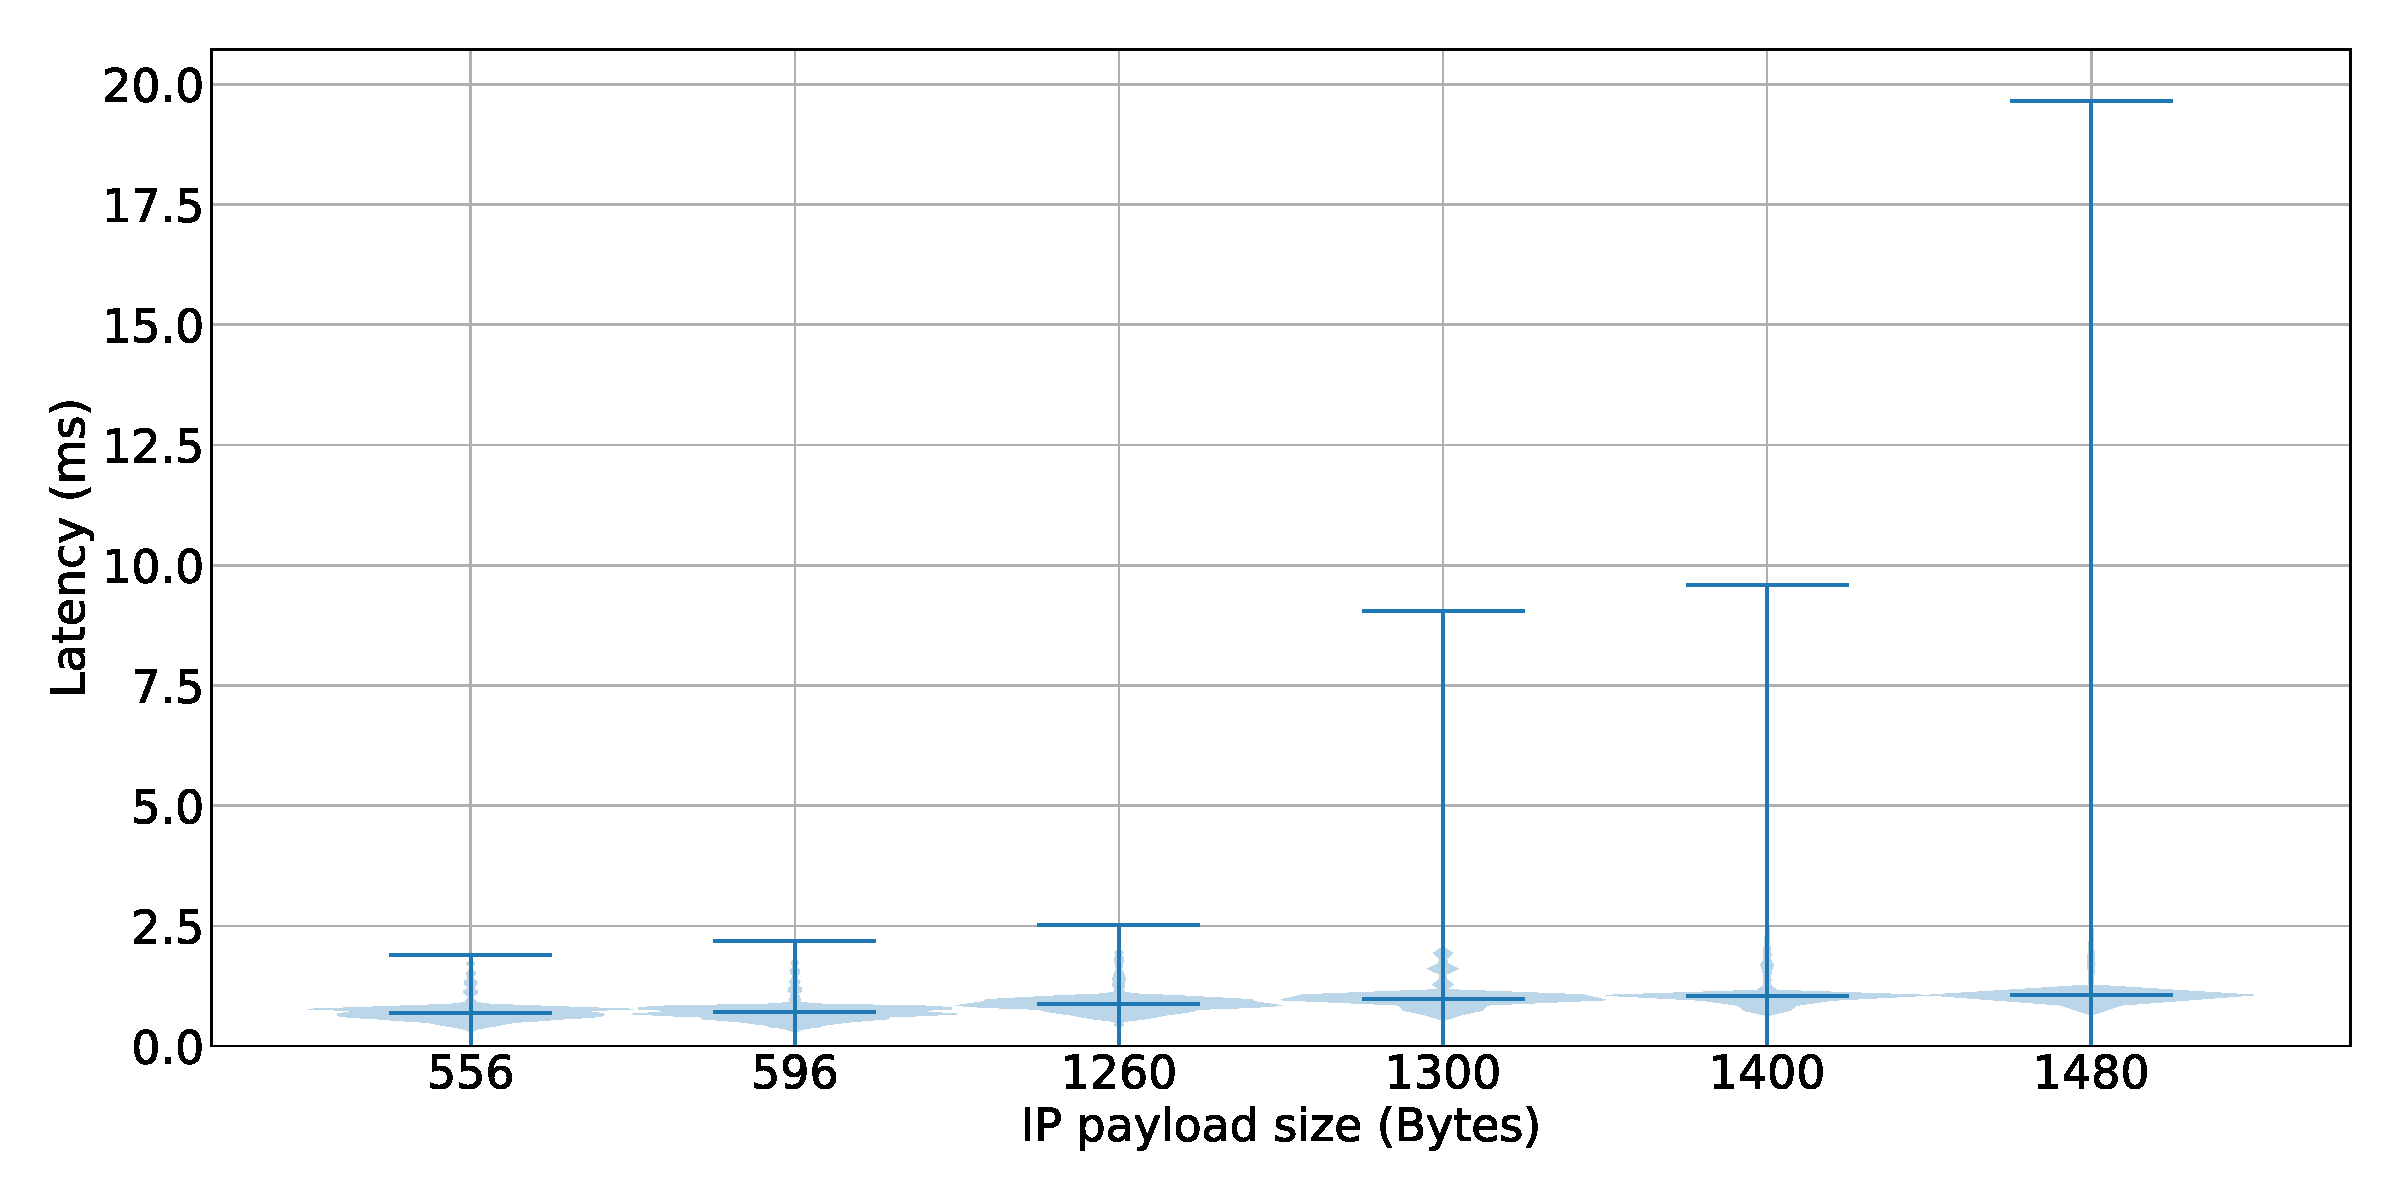
\includegraphics[draft=false,width=0.9\textwidth]{figures/Graphs/graph-4-mtu/latencies.pdf}
	\caption{Latencies for varying payload sizes without any tunnel protocol and all other parameters set to zero}
	\label{fig:graph-4-mtu-latencies}
\end{figure}
\begin{figure}[t!]
	\centering
	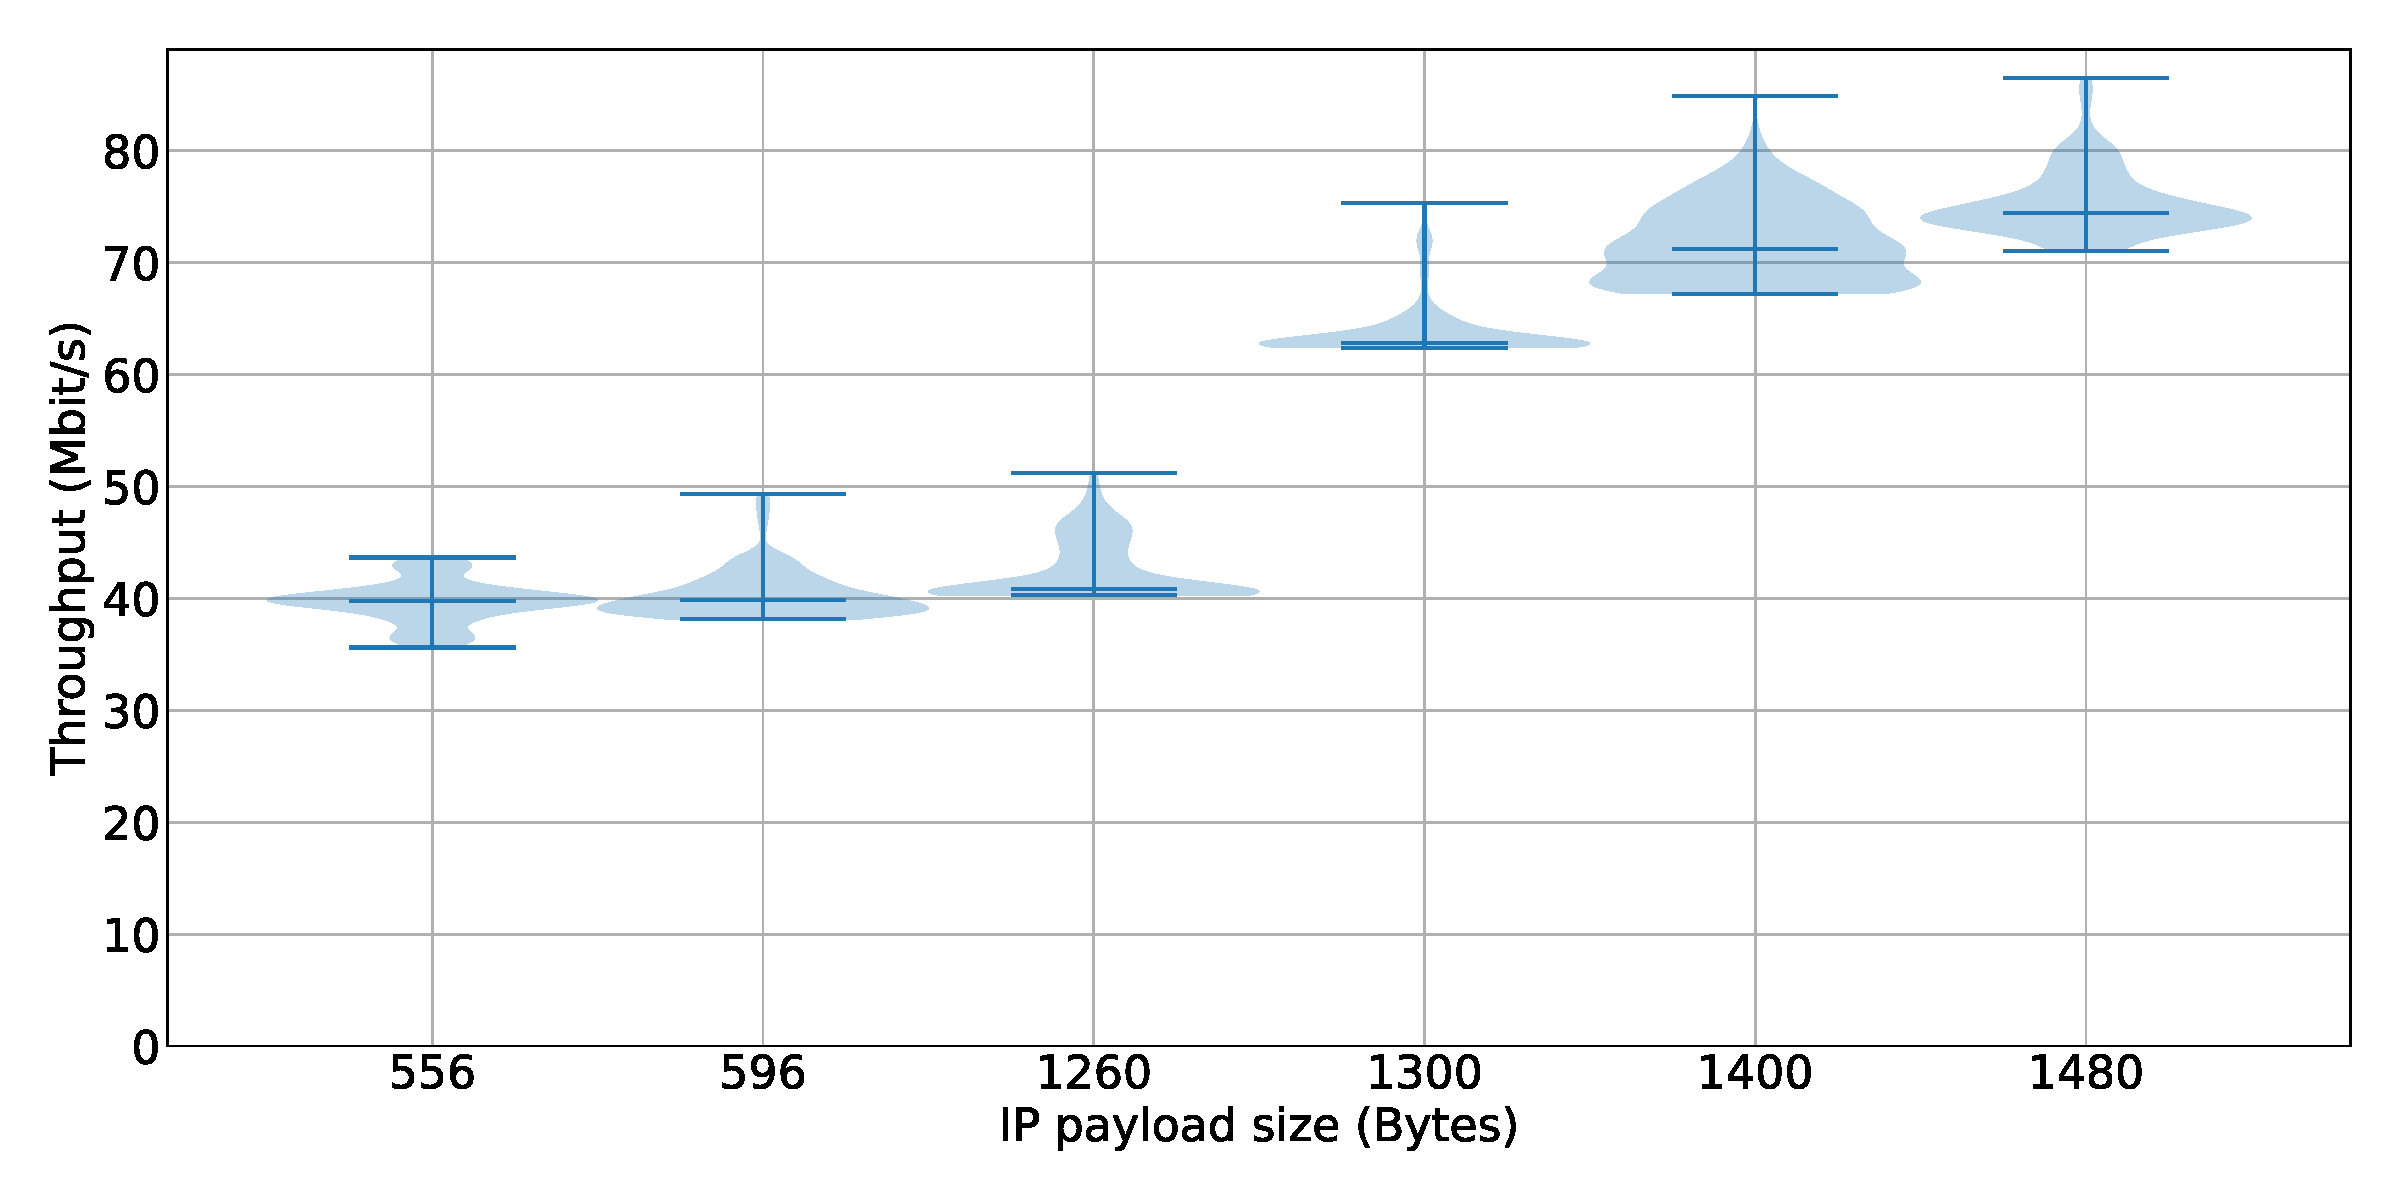
\includegraphics[draft=false,width=0.9\textwidth]{figures/Graphs/graph-4-mtu/throughput.pdf}
	\caption{Throughput for varying payload sizes without any tunnel protocol and all other parameters set to zero}
	\label{fig:graph-4-mtu-throughput}
\end{figure}
\begin{figure}[t!]
	\centering
	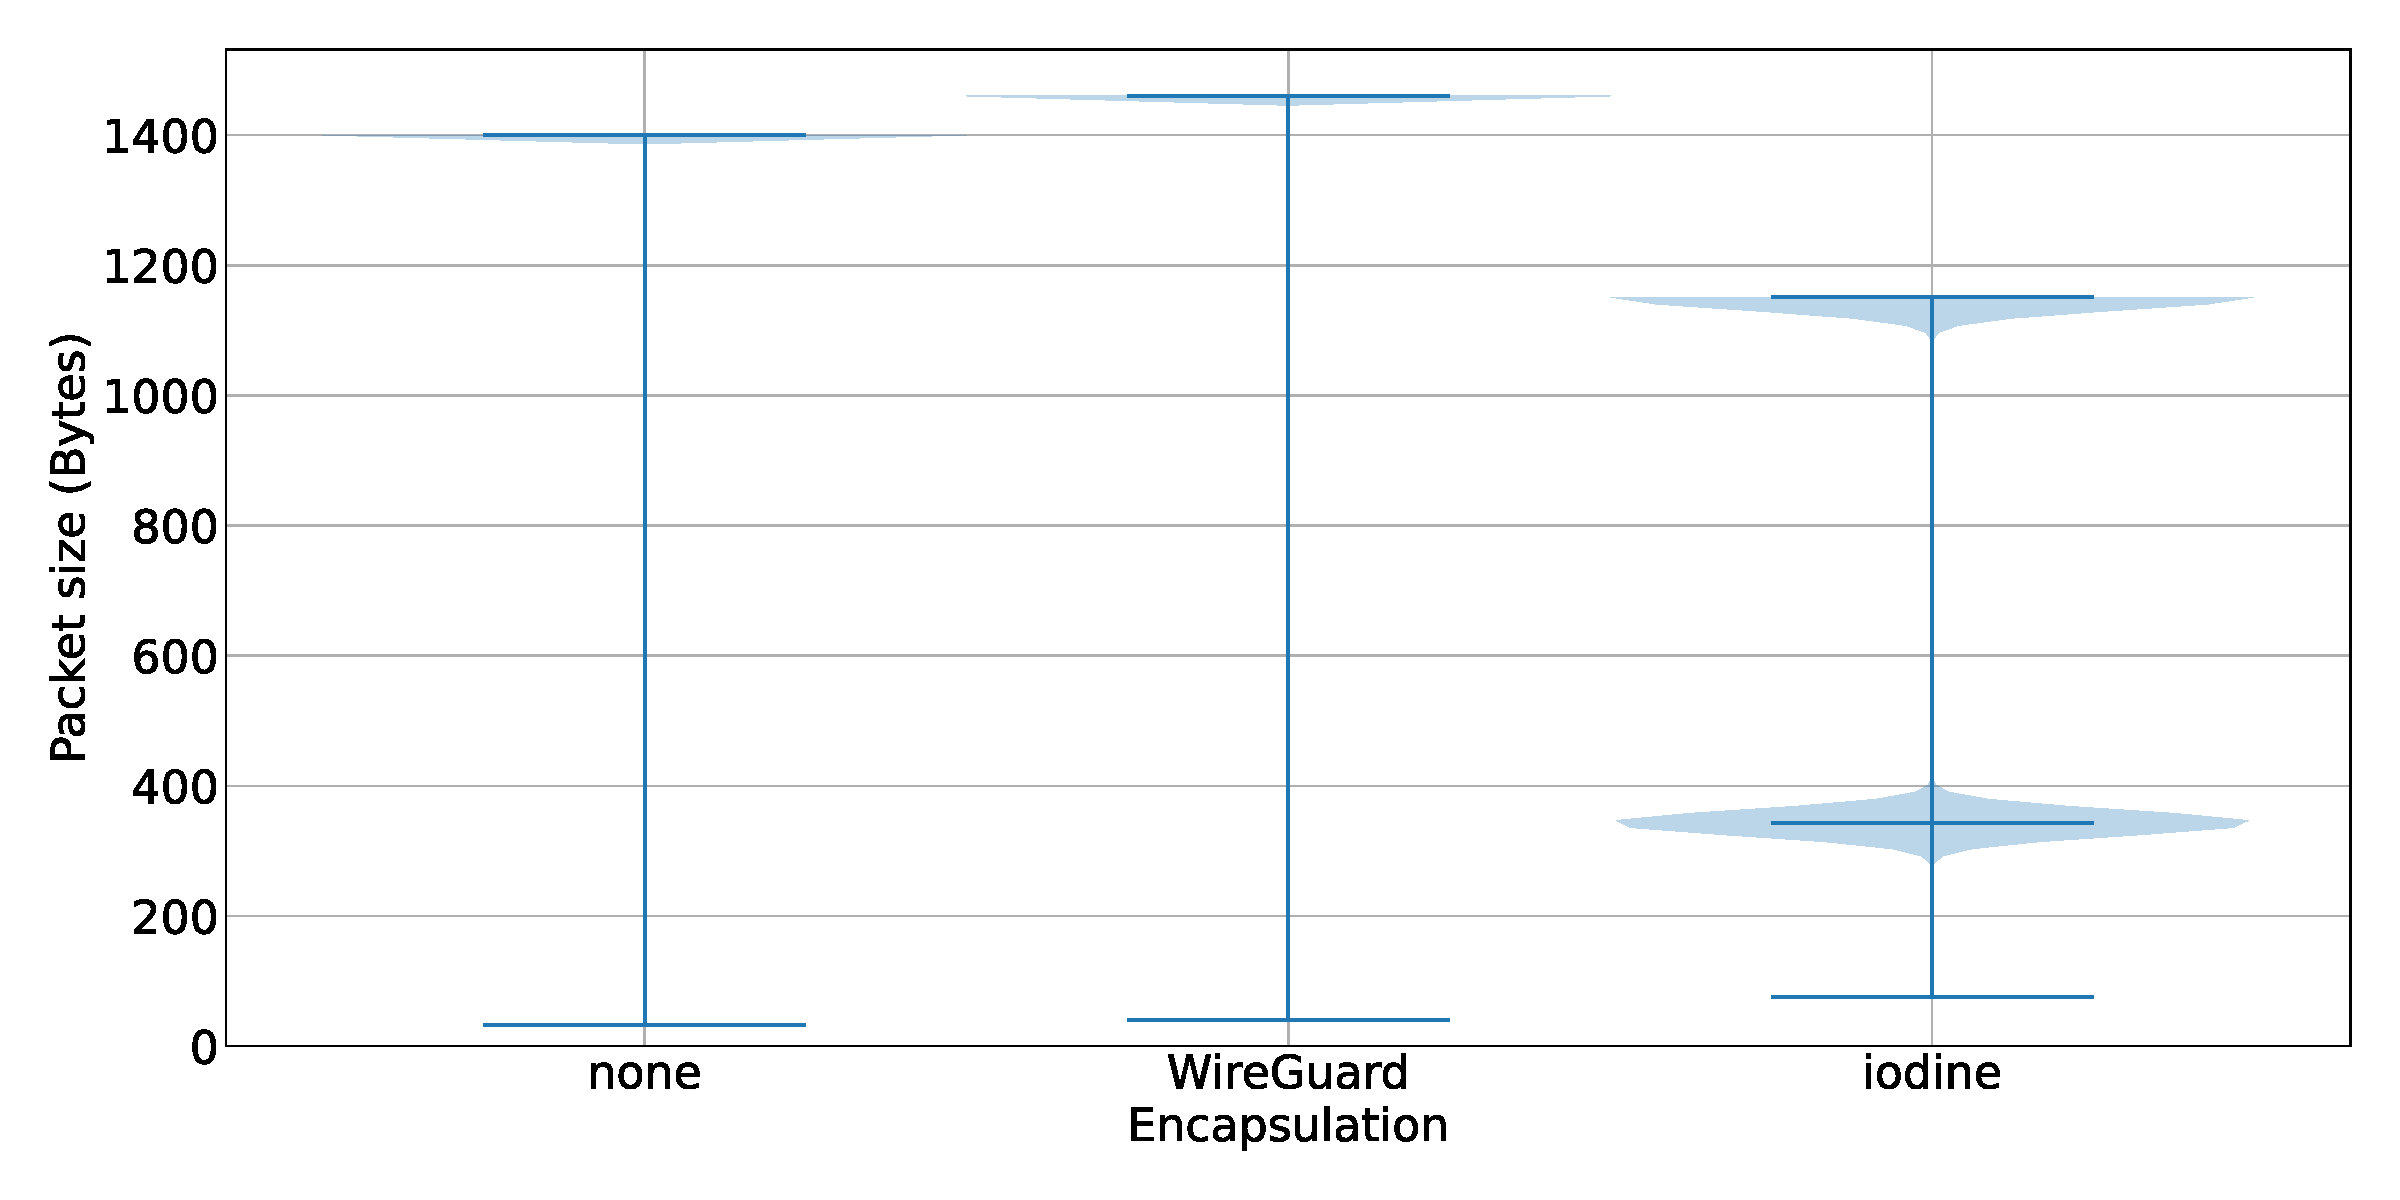
\includegraphics[draft=false,width=0.9\textwidth]{figures/Graphs/graph-6-three-protocols/packet_size.pdf}
	\caption{Packet size for varying tunnel protocols, 1400 IPv4 payload size, 0.1\% loss}
	\label{fig:graph-6-three-protocols-size}
\end{figure}

The x-axis represents the different measurement runs (each varying a parameter of interest), and the y-axis represents the corresponding metric.
All graphs, except for the latency and packet sizes, use the data from the buckets above to show a distribution of values rather than e.g., only the mean value.
An example of this type of graph can be seen in \Cref{fig:graph-4-mtu-throughput}.

\noindent\textbf{Latency:} A violin plot displays the distribution of latency across all measurement runs.
This visualization combines the features of a box plot (showing median, quartiles, and outliers) with a kernel density estimation (showing the shape of the distribution).
This helps us compare the overall latency distribution across different parameter values.

\noindent\textbf{Packet Duplication Ratio:} A violin plot shows the ratio of duplicate packets to the total number of packets sent for each measurement run.
This visualization allows us to assess how the duplication rate changes with different parameter values.

\noindent\textbf{Packet Drop Ratio:} A violin plot displays the ratio of dropped packets to the total number of packets sent for each measurement run.
This helps us understand how packet loss is affected by the varied parameter.

\noindent\textbf{Packet Size:} A violin plot shows the distribution of packet size.
The value refers to the IP payload size outside of the tunnel.
This is very useful for observing if fragmentation took place.
If packets are fragmented, multiple different packet sizes will be common.

\noindent\textbf{Throughput (with and without overhead):} Two violin plots are used to show throughput, one including overhead added by the protocol and the other excluding it.
This comparison helps visualize the overhead introduced by the protocol and how it affects the effective throughput.


Notably, in \Cref{fig:graph-4-mtu-latencies} we observe that latency remains largely constant with varying packet sizes, except for a drastic increase in tail latency, which was an unexpected finding.

In \Cref{fig:graph-4-mtu-throughput} we see that the throughput decreases with lower IP payload size.

\Cref{fig:graph-6-three-protocols-size} shows that WireGuard adds some overhead to each packet, as expected.
iodine fragments the packets since our IP packets (1420 bytes) are larger than the MTU of the tunnel interface.

Rather than only a handful of combinations of parameters, as described in \Cref{chap:methodology}, we tested many more for experimentation.
In the beginning we even tested the Cartesian product of all parameters.
This fact combined with several slightly different versions of our test setup, lead us to collect about 5 TB of packet captures, which compress to about half the size of that using the zstd compression algorithm in Btrfs.


%%% Local Variables:
%%% TeX-master: "thesis"
%%% End: